%----------------------------------------------------------------------------
%\chapter{\Kubernetes}
%\label{sec:Kubernetes}
%----------------------------------------------------------------------------
\chapter{Kubernetes}
\label{sec:Kubernetes}
A félévben végzett munka jelentős mértékben támaszkodik a Kubernetes (K8s) rendszerre, így annak ismertetése szükségszerű. 

%----------------------------------------------------------------------------
\section{Motivációja}
%----------------------------------------------------------------------------
Ahogy egyre többen kezdték megismerni és használni a konténerizációs technikákat, mint például a Docker, úgy egyre tolódott át az üzemeltetési oldal is ilyen irányba. Ezek után nem  az jelentette a kihívást, hogy az egyes alkalmazásokat egy dedikált virtuális gépen kellett beüzemelni és elindítani. Az új igények szerint az alkalmazásunk egyes részeit egymástól függetlenül kellett konténerekben futtatni. Ezáltal sokkal több kisebb részegységre kellett figyelni, ami jelentősen több feladattal jár, mint a korábbi gépek kezelése. 

Ezzel a problémával találkozott a Google is és kezdődött egy platform fejlesztése, ami képes a fenti feladatok megoldására. Eleinte ez a \textit{Borg}\citep{Borg} nevet viselte. Ezt 2014-ben a Google nyílt forráskódúvá tette immáron Kubernetes néven. A projektet a \textit{Cloud Native Computing Foundation (CNCF)} vette gondozásába. Innentől kezdve bárki szabadon elérheti és bele is fejleszthet. Az elmúlt 6 év alatt hatalmas fejlődésen ment keresztül és már a $22$.-ik kiadásánál tart.

%----------------------------------------------------------------------------
\section{Felépítése}
%----------------------------------------------------------------------------

%TODO erőforrások: CPU és memoria
\subsection{Erőforrások}
%----------------------------------------------------------------------------

\subsection{Objektumok}
%----------------------------------------------------------------------------
A Kubernetes egyik erőssége, hogy az átlagos felhasználás esetében nem kell törődni a rendszer felépítésével, hiszen nekünk csak deklaratív módon meg kell létrehozni és kezelni bizonyos erőforrásokat, objektumokat.
  
\paragraph{Pod (kapszula)}
A Kubernetesben megjelenő legkisebb egység. Általában egy konténert futtat, de lehetőségünk van több konténer futtatására is. Általánosságban elmondható, hogy rendszeresen létrejönnek és rendszeresen törölve is lesznek ezek az objektumok, tehát nem tartós életűek. Ez az egész rendszernek tud adni egy 

\paragraph{ReplicaSet} 
Az ő feladata, hogy bizonyos \textit{Podból} megfelelő számú egység fusson. Ennek értelmében, ha az egyik \textit{Pod} meghibásodik és megáll, akkor helyette egy újat fog létrehozni. Ezáltal biztosított, hogy mindig a megfelelő számú egység fogja fogadni a beérkező kéréseket és nem kell manuálisan monitorozni a státuszukat.

\paragraph{Deployment}
Mivel \textit{kapszulák} túl kicsi részei a teljes alkalmazásnak és életük sem kiszámítható ezért nem kifizetődő ilyen módon kezelni a rendszerünket. Erre találták ki a \textit{Deploment} objektumot, ahol meg tudjuk adni, hogy milyen \textit{Podok} jöjjenek létre, illetve beállíthatjuk a hozzájuk kapcsolódó \textit{ReplicaSet} értéket is. Ezáltal lehetőségünk van absztrakt szinten deklaratívan módon megadni a kívánt rendszer tulajdonságait.

\paragraph{Service}
A korábban említett objektumokkal már meg tudunk valósítani bizonyos funkciókat, viszont ezt szeretnénk a klaszteren belül és kívülre is elérhetővé tenni. Erre találták ki \textit{Servicet}. Ezen keresztül könnyen el tudjuk érni az azonos szolgáltatást nyújtó \textit{kapszulákat} és nem kell az alkalmazás logikában számontartani az ő elérhetőségeiket. Ez ugye különösen nehéz feladat lenne, hiszen a készenléti idejük is elég változó lehet, mivel folyamatosan jönnek létre és törlődnek.

\paragraph{CustomResourceDefinition (CRD)}
%TODO

%----------------------------------------------------------------------------
\section{Skálázás}
%----------------------------------------------------------------------------
A felhős infrastruktúra egyik legcsábítóbb előnye, hogy az alkalmazásunk képes adaptálódni a külvilág felől érkező kérésekhez. Ez azt jelenti, hogy ha több felhasználót kell egyszerre kiszolgálni, akkor a rendszer automatikusan növeli a kiszolgálásra fordított erőforrások mennyiségét. Ezzel a megoldással elérhetjük, hogy a végfelhasználó ne vegyen észre minőségbeli csökkenést és a kevésbé intenzív időkben pedig nem foglalunk feleslegesen erőforrást, ami az üzemeltetőnek is jól belátható anyagi érdeke.
 
Alapvetően két különböző skálázási módszert lehet elkülöníteni. Az egyik a vertikális, míg a másik a horizontális skálázás. Ezekről a későbbiekben bővebben lesz szó. 

\subsection{Horizontális skálázás}
%----------------------------------------------------------------------------
A két skálázási mód közötti különbséget mutatja a \refstruc{fig:scaling}. Jobb oldalon látható megoldás az úgynevezett horizontális skálázás (másik nevén: scaling out). Ebben az esetben arról van szó, hogy a megnövekedett igények kiszolgálásához több azonos egységet hozunk létre. Az összes egység azonos erőforrás felhasználással rendelkezik és a beérkező kérések köztük lesznek szétosztva. 
A megoldás egyik legnagyobb előnye, hogy elég könnyű alkalmazni, a Kubernetes rendszere is alapértelmezettként támogatja. Hátrányánál meg lehet említeni, hogy több egység között oszlanak meg a beérkező kérések így nem biztos, hogy azonos egységnél köt ki egy felhasználó két különböző kérése. 

\subsubsection{Automatikus horizontális skálázás}
%----------------------------------------------------------------------------
Egy egyszerű példán keresztül szeretném bemutatni a Kubernetes beépített, automatukis horizontális skálázóját (HPA). Az automatikus skálázónak meg lehet adni, hogy milyen célértéket szeretnénk kapni. Például, hogy a futtatott \textit{Pod} által felhasználható CPU mennyiség milyen szinten legyen kihasználva. Jelenleg ilyen megkötést a memória és processzor felhasználásra lehet tenni, de tetszőlegesen létrehozhatunk saját metrikát. 

Az algoritmus folyamatosan lekérdezi a metrikák aktuális értékét és a \ref{hpa_algo} egyenlet alapján meghatározza az éppen szükséges replika számot. Ezzel a számított értékkel frissíti a \textit{Pod} replika számát, amit így a replikációért felelős kontroller észlel és megpróbálja elérni a kívánt állapotot. Ezzel módszerrel megvalósítható fel- és leskálázás is.

\begin{equation}
\label{hpa_algo}
desiredReplicas = \lceil currentReplicas * ( currentMetricValue / desiredMetricValue ) \rceil
\end{equation}

A folyamat szemléletesebb, ha konkrét példán nézzük meg működését. Ehhez először létre kellett hozni egy alkalmazást, amit tudunk majd skálázni. Ehhez egy egyszerű webszervert használtam, ami minden beérkezett kérés esetén egy CPU intenzív műveletet hajt végre. Miután létrejött a szükséges \textit{Deployment} és \textit{Service} utána létre lehetett hozni az automatikus skálázót. Ennek a forráskódja látható a \ref{hpa_example} kódrészlet tetején. Be lehet állítani, hogy mi legyen a minimális és maximális replika, ami között tud skálázni. Illetve meg kell a szabályt is, hogy mire kell figyelni. A példában látható, hogy $50\%$-os CPU felhasználást szeretnénk elérni. Fontos, hogy alapvetően a metrikákat a skálázó egy úgynevezett metrika szervertől gyűjti be, amit külön el kell indítani, mert alapértelmezettként nem fut a Kubernetesben.

Ha létrehoztuk a skálázót, ki is lehet próbálni. Ehhez egy \verb+bash+ szkript segítségével állandó forgalmat generálunk és figyeljük meg, hogyan változik a kapszulák száma és ezzel összefüggően az egyes egységek CPU felhasználása. Kezdetben $1$ darab \textit{Pod} végezte az összes beérkező kérés kiszolgálását, ami így a célértéknél 3-4-szer több processzort használt. A korábban mutatott képlet alapján, a felső egész részt vesszük és a jelenlegi replikaszám 4-szeresére skálázunk. \\
 
\lstset{caption=Automatikus horizontális skálázás folyamata, label=hpa_example}
\lstinputlisting{figures/hpa_example.sh}


\subsection{Vertikális skálázás}
%----------------------------------------------------------------------------
A skálázási megoldások közül a másik megoldás a \refstruc{fig:scaling} bal oldalán látható. Ezt vertikális skálázásnak (másik nevén: scaling up) hívnak. Ebben az esetben a kiszolgáló egységek számát nem módosítjuk, hanem az általuk felhasználható erőforrások mennyiségét növeljük. Ilyen példa, amikor plusz memóriát rakunk a számítógépbe, vagy erősebb processzorra cseréljük a meglévőt.
Kubernetes jelenleg még nem támogatja alapértelmezettként ezt a funkciót, de egyszerűen használatra lehet bírni. Előnye a megoldásnak, hogy a korábbi félévek munkái alatt azt figyeltük meg, hogy a vizsgált alkalmazásaink ezzel a stratégiával azonos erőforrás felhasználás mellett jobb eredményeket értek el.\citep{bscThesis} 
%TODO le kell állítani jelenleg

% Skálázás módjai ábra -------------------------------------------------------
\begin{figure}[!ht]
\centering
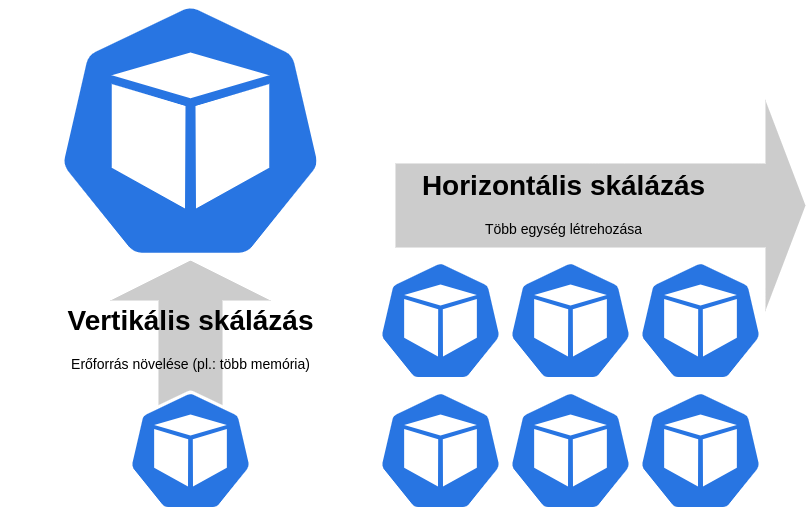
\includegraphics[width=150mm, keepaspectratio]{figures/scaling_types.png}
\caption{Vertikális és horizontális skálázás}
\label{fig:scaling}
\end{figure}
